To purpose of splitting the back-end scripts from the front-end interface is to separate the functionality from the graphical interface, following a model-view pattern where the model is the back-end scripts which manages the logic and data and the view is the front-end interface. The backend was chosen to be written in Python, due to it having more support and separated libraries for SSH and Telnet compared to Java. For the back-end scripts, I separated the functionality using two scripts, one for the quick scanning utility and the other for advanced scanning.

\subsection{Backend Structure}

\begin{figure}[h]
	\centering
	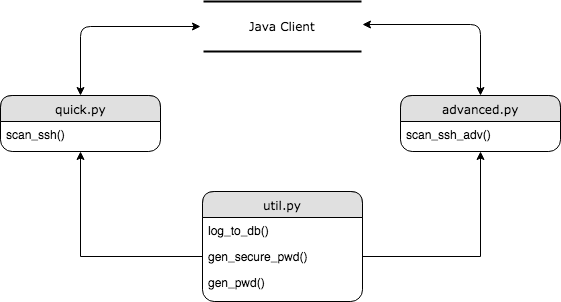
\includegraphics[width=1\linewidth]{img/backend_structure.png}
	\caption{Back-end Structure}
\end{figure}

As seen in the above image, the functionality is separated into quick and advanced scanning scripts. Initially the scripts both contained the utility functions as described by \textit{util.py}, but were refactored to increase the degree of modularity in the code.

\vspace{0.5cm}

There are two functions for password generation which are \textit{gen\_pwd()} and \textit{gen\_secure\_pwd()}. The \textit{gen\_pwd()} function generates a \textbf{cryptographically secure} 16 character long password, made up of letters, numbers and symbols. It ensures a cryptographically secure password by using the \textit{secrets} module to select a random character, generated by SystemRandom (which generates the number from sources provided by the operating system), from the alphabet shown in Listing 4.3.

\begin{lstlisting}[language=Python, caption=Password Alphabet]
alphabet = string.ascii_letters + string.digits + string.punctuation
\end{lstlisting}

The second function, \textit{gen\_secure\_pwd()} is used to ensure that the password ultimately generated contains at least one uppercase letter in the password, following the Linux root password standard.

\subsection{Logging}

As shown in Figure 4.2, the utility script consists of a logging function, which sends the resulting scan log to the database attached with the UUID of the user who performed the scan.

\vspace{0.5cm}

The Java client uses a \textit{JEditorPane} to display scan results, which supports HTML 3.2. This is an outdated version of HTML, but provides more than enough elements to support the requirements of displaying scan logs. Therefore during the scan, a list of HTML elements is collected along with relevant information for each part of the scan. This list is then joined together and output to the \textit{log\_to\_db()} function to store the scan log. Appendix B.1 shows an example scan log for an SSH scan.

\subsection{Scanning}

Miraihilate's scanning capability is divided into quick scanning and advanced scanning. The aim of the quick scan utility is to enable a simple scan to run on a network range once the client has started, whilst the advanced scanning allows users to set the timeout for scanning and provide extra commands to the devices. Once a scan has completed, the data will be sent to the database and the client will update to display the latest scan results.

\subsubsection{SSH Scanning}

The SSH scanning function scans a specified network range and attempts to bruteforce into device root accounts found on the IP address range, using a default list of username/password combinations through an SSH connection. It loops through a list of ip addresses specified by an IP address and a CIDR suffix and then tries to establish an SSH connection to the device, trying each of the username/password combinations. If a connection is made it will look at the parameters sent to the scan, relative to whether it was a quick or advanced scan, and perform its respective function such as changing the password of an infected device.

\subsubsection{<Telnet Scanning?>}

Note: This has no effect on usability, but if there is time to ultimately implement Telnet functionality, I can fill this in.
